\section{Transformer模型简介}\label{sec-3}

由于在课程中已有对Transformer模型的深入讨论,因此这里我们只简要介绍注意力机制和Transformer模型的架构,不做过多详细的解释。

\subsection{注意力机制}

我们这里重点介绍自注意力机制、多头注意力机制和交叉注意力机制。

\subsubsection{自注意力机制}

自注意力(Self-Attention),也称为内部注意力,是一种让序列中的每个位置关注序列中其他所有位置的方法。通过计算查询(Query)、键(Key)和值(Value)向量之间的相似度得分,模型可以加权汇总这些值,以产生序列中每个元素的新表示。这有助于捕捉序列内的长期依赖关系。

简单来说,对于一个形状为$(s,h)$的输入向量$X$,其中$s$代表序列长度,$h$代表词嵌入维度,我们提供三个转换矩阵$W_Q,W_K,W_V$,形状均为$(h,h)$,计算
$$
Q = XW_Q , \ 
K = XW_K , \ 
V = XW_V X, \ \ \ \text{形状均为}(s, h)
$$
得到三个形状均为$(s,h)$的向量,分别表示查询、键和值。之后我们计算注意力得分
$$
O = \text{softmax}(\frac{QK^T}{\sqrt{h}}) V, \ \ \ (s,h)
$$

\subsubsection{多头注意力机制}
多头注意力(Multi-head Attention)是指并行运行多个自注意力机制,每个都有独立的参数集。这使得模型可以在不同的子空间中多次关注输入的不同方面,增强模型对不同位置信息的理解能力。最终,所有头的输出被连接起来,并通过一个线性变换进行投影。

在实现上,假设一共有$a$个头,每个头提供自己的转化矩阵$W_Q^i,W_K^i,W_V^i$,形状均为$(h, \frac{h}{a})$,以便于我们计算出每个头最后的注意力得分后,能够将输出拼接成和输入$X$维度相同的矩阵。同时,我们增加一个将每个头的注意力分数$Z_i,(s,\frac{h}{a})$连接起来的线性层$W_O,(h,h)$,充分获取所有头的信息。
$$
Q_i = XW_Q^i , \ 
K_i = XW_K^i , \ 
V_i = XW_V^i ,  \ \ \ \text{形状均为}(s, \frac{h}{a}),
$$
$$
Z_i = \text{softmax}(\frac{Q_iK_i^T}{\sqrt{\frac{h}{a}}}) V_i, \ \ \  (s, \frac{h}{a}),
$$
$$
O = [Z_1, Z_2,\cdots , Z_a] W_O,  \ \ \ (s, h),
$$

\subsubsection{交叉注意力机制}
交叉注意力(Cross Attention)用于编码器-解码器结构中,使解码器能够关注到编码器产生的所有位置。具体来讲,编码器提供输入$X$,解码器提供输入$Y$,形状均为$(s,h)$,通过下述过程得到
$$
Q = XW_Q , \ 
K = YW_K , \ 
V = YW_V , \ \ \ \text{形状均为}(s, h),
$$
也就是说,在交叉注意力机制中,$Q$来自编码器输入,$K,V$来自解码器输入。

这是翻译任务等序列到序列问题的关键,其中解码器需要根据源序列的信息生成目标序列。

\subsubsection{掩码}

这里只介绍用于解码器自注意力机制的掩码。由于在训练时,我们训练的目标是预测解码器输入的后续序列,模型只能关注生成内容的当前位置之前的信息,不能提前预知未来信息,因此需要对当前位置之后的信息提供掩码。

\subsection{Transformer模型}

Transformer模型摒弃了传统的循环神经网络(RNN)和卷积神经网络(CNN)结构,完全依靠注意力机制来处理序列间的依赖关系。模型主要由编码器和解码器两部分组成,在自注意力机制和交叉注意力的机制上,还增加了
\begin{itemize}[itemsep=-5pt, leftmargin=4em]
    \item \textbf{嵌入层}\  将输入的离散符号(如单词、字符等)映射为连续的词向量,使模型能够处理语言数据并捕捉语义信息;
    \item \textbf{位置编码}\  为输入序列的每个元素添加位置信息,使模型能够感知序列中单词的位置顺序,弥补自注意力机制无法天然感知顺序的缺陷;
    \item \textbf{前馈神经网络层}\  对经过自注意力机制处理后的信息进行全连接操作,进一步转换和提取特征,为后续的输出做准备;
    \item \textbf{残差连接} \ 将输入直接添加到输出上,为梯度提供直接的传递路径,避免梯度消失或爆炸,使模型能够训练更深的网络结构;
    \item \textbf{层归一化} \ 对每一层的输出进行归一化处理,稳定训练过程,减少内部协变量偏移现象,提高模型的收敛速度和训练稳定性;
    \item \textbf{预测层}\  将最终的注意力输出映射为具体的概率分布。
\end{itemize}

在此基础上,构建两个子模块:

\begin{itemize}[itemsep=-5pt, leftmargin=4em]
    \item \textbf{编码器}\  由一系列相同的层堆叠而成,每一层的构成依次为:多头自注意力机制、残差连接和层归一化、全连接前馈神经网络、残差连接和层归一化。
    
    \item \textbf{解码器}\  同样由一系列相同层构成,每一层的构成依次为:多头自注意力机制、残差连接和层归一化、多头交叉注意力机制、残差连接和层归一化、全连接前馈神经网络、残差连接和层归一化。
\end{itemize}

具体的架构如图\ref{fig:transformer}所示。

\begin{figure}[htb]
    \centering
    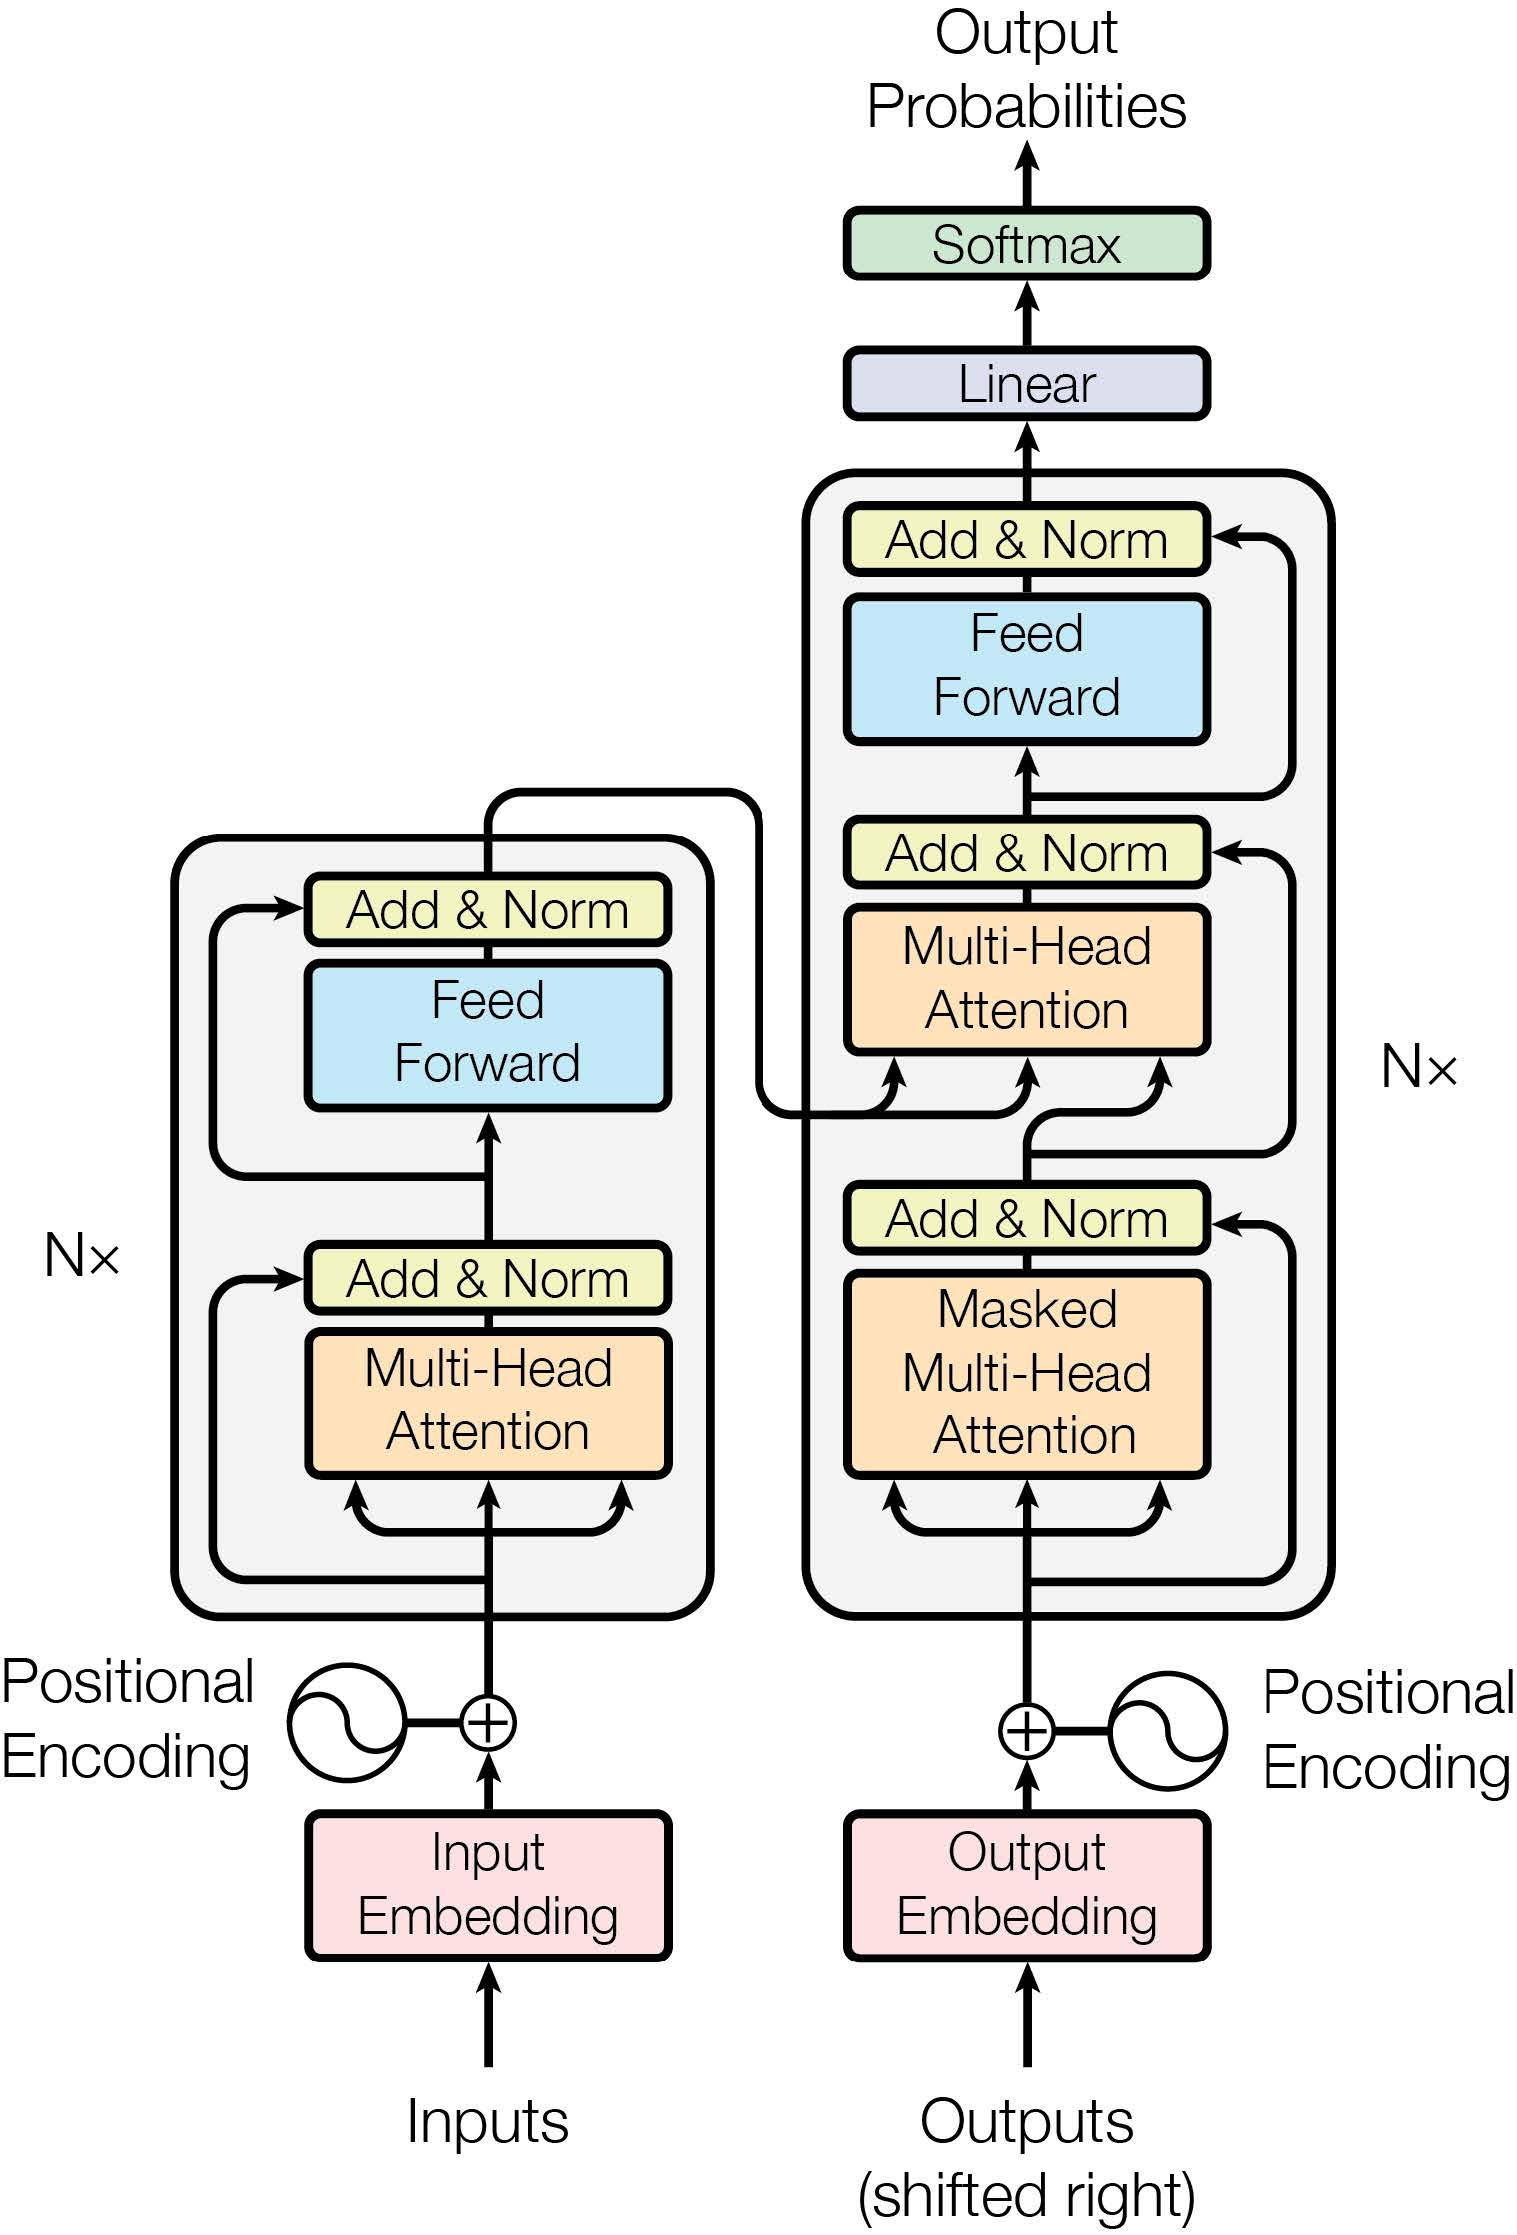
\includegraphics[width=0.45\linewidth]{img/transformer.jpg}          
    \caption{Transformer架构图}
    \label{fig:transformer}
\end{figure}
